
% =====================================================================
\section{Experiments}
\label{sec:exp}
% =====================================================================

We organize our experiments into five analyses. All experiments use the same EG3D generator pretrained on FFHQ~\cite{StyleGAN2}. VLM experiments use Qwen3-VL-2B with 4-bit quantization on an NVIDIA RTX 5060 Laptop GPU.

% ---------------------------------------------------------------------
\subsection{Cross-Attention Spatial Grounding}
\label{sec:exp_attention}
% ---------------------------------------------------------------------

\begin{figure}[t]
    \centering
    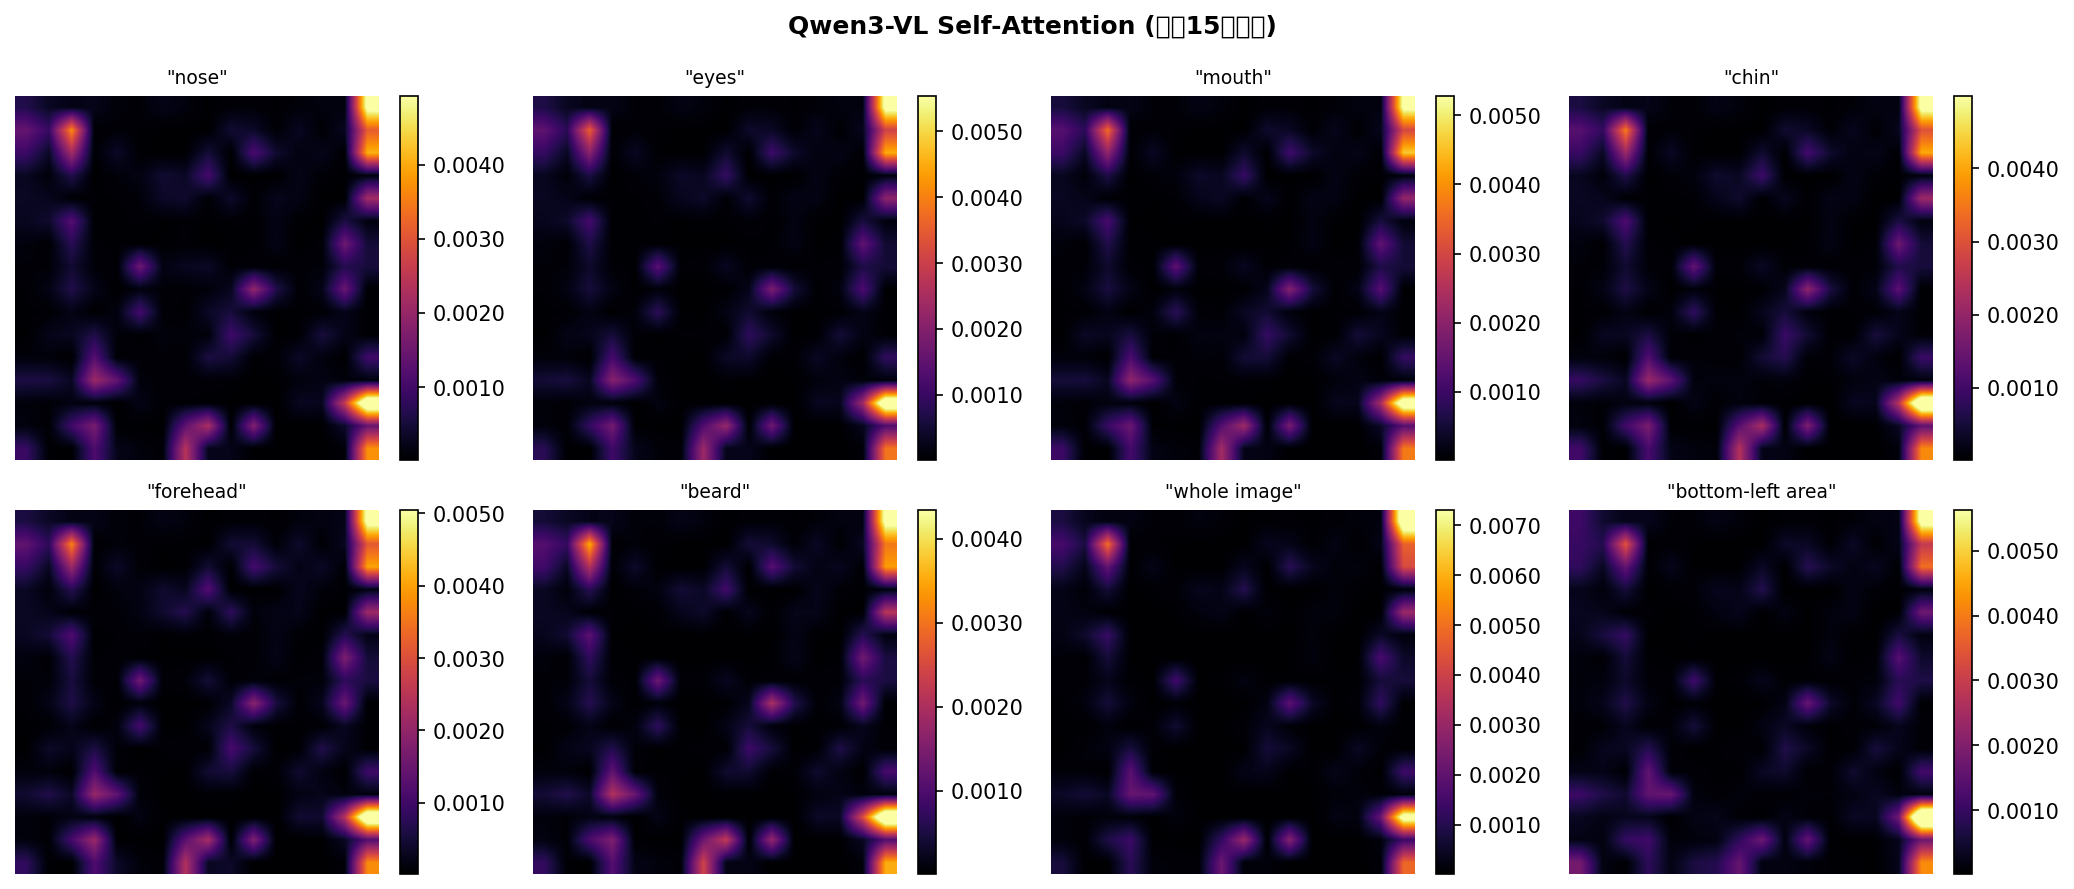
\includegraphics[width=\linewidth]{figures/heatmap_right15.png}
    \caption{Visualization of Qwen3-VL self-attention maps for eight queries. All queries produce near-identical attention distributions on the same face image.}
    \label{fig:heatmap}
\end{figure}

\begin{figure}[t]
    \centering
    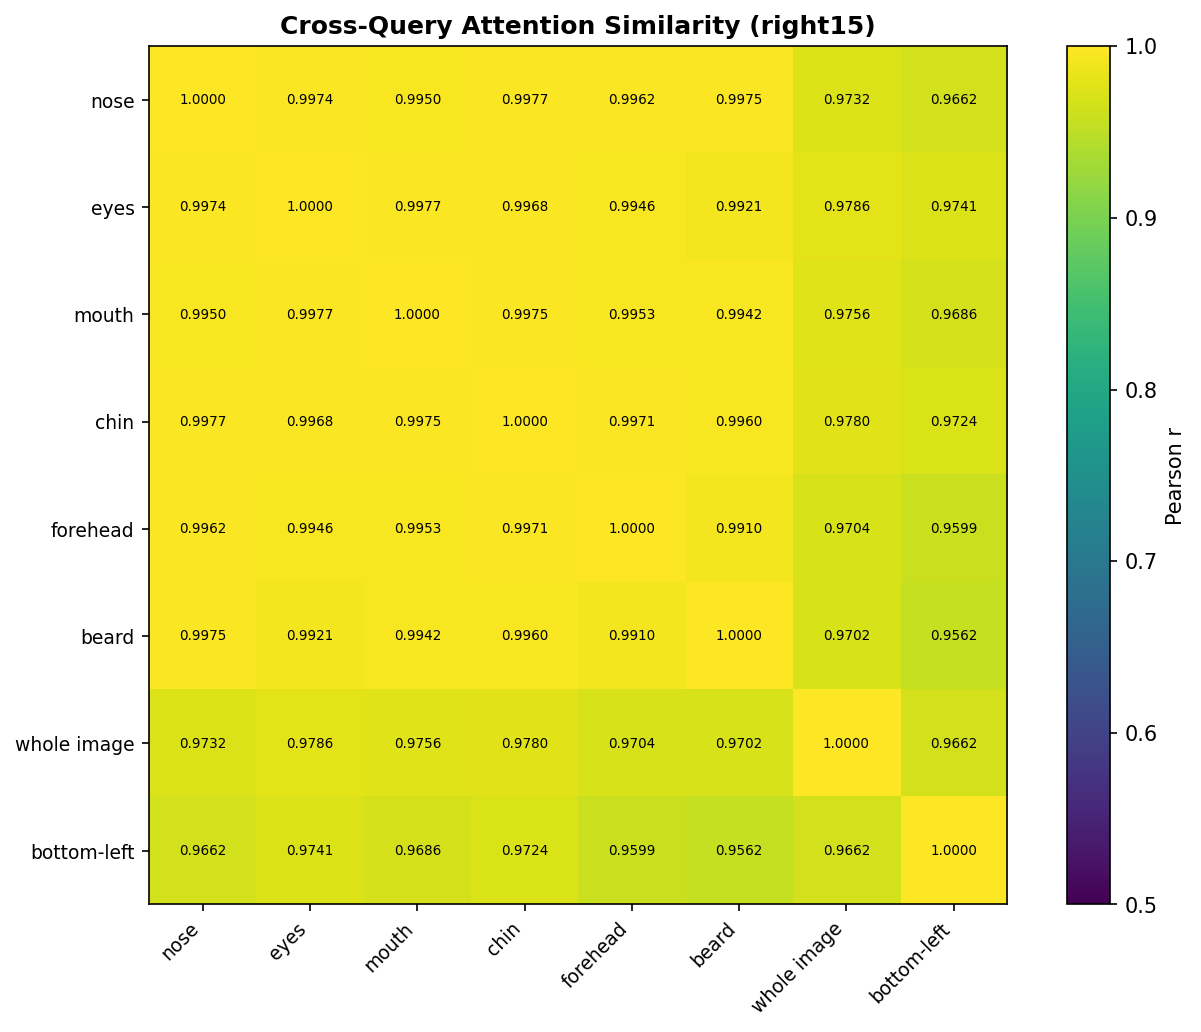
\includegraphics[width=\linewidth]{figures/similarity_right15.png}
    \caption{Cross-query similarity matrix of attention maps. All Pearson r values exceed 0.999, indicating that VLM self-attention fails to differentiate facial features.}
    \label{fig:sim}
\end{figure}

\textbf{Setup.} We input a face image alongside text queries such as ``describe the nose'', ``describe the eyes'', and control queries (``whole image'', ``bottom-left area''). We extract the self-attention weights from the last three LLM layers, average across heads and layers, and measure the attention from the query tokens to the 16$\times$16 visual token grid.

\textbf{Results.} Figure~\ref{fig:heatmap} visualizes the attention maps; Figure~\ref{fig:sim} shows the Pearson correlation matrix. Every query---whether a specific facial feature or a control phrase---produces an attention map with correlations exceeding 0.9999 (Table~\ref{tab:sim_stats}). The minimum observed correlation is 0.99968 (between ``beard'' and ``bottom-left''), which is at the level of floating-point noise. This demonstrates that Qwen3-VL's self-attention cannot spatially distinguish facial features, rendering it unsuitable for fine-grained face control tasks.

\begin{table}[t]
\centering
\caption{Cross-query attention similarity statistics (Pearson r across all pairs).}
\label{tab:sim_stats}
\begin{tabular}{lcc}
\toprule
Query group & Mean r & Min r \\
\midrule
Face features (6 queries) & $>$0.9999 & 0.99968 \\
Control queries (2 queries) & $>$0.9999 & 0.99968 \\
Face vs. control & $>$0.9999 & 0.99968 \\
\bottomrule
\end{tabular}
\end{table}

% ---------------------------------------------------------------------
\subsection{Embedding Sensitivity}
\label{sec:exp_emb}
% ---------------------------------------------------------------------

\textbf{Setup.} We generate 10 prompts differing only in the target angle: ``A person looking to the right at $X$ degrees'' for $X \in \{0, 10, \ldots, 90\}$. For each prompt, we extract the VLM hidden state (2048-dim) and the CLIP embedding (512-dim). We compute pairwise cosine similarity matrices and measure two metrics: adjacent-angle similarity (10\textdegree~apart) and far-angle similarity (40\textdegree~or more apart). The discriminability is defined as the difference between these two.

\begin{table}[t]
\centering
\caption{Embedding sensitivity to fine-grained angle descriptions.}
\label{tab:sensitivity}
\begin{tabular}{lcc}
\toprule
Metric & VLM 2B & CLIP 63M \\
\midrule
Mean pairwise similarity & 0.9962 & 0.9469 \\
Adjacent (10\textdegree) similarity & 0.9976 & 0.9752 \\
Far (40\textdegree+) similarity & 0.9948 & 0.9293 \\
Discriminability (adj.~$-$ far) & \textbf{0.0028} & \textbf{0.0459} \\
\bottomrule
\end{tabular}
\end{table}

\textbf{Results.} As shown in Table~\ref{tab:sensitivity}, VLM hidden states exhibit a mean pairwise similarity of 0.9962, indicating that all 10 angle descriptions map to nearly identical representations. The discriminability is only 0.0028, meaning the model cannot meaningfully distinguish 10\textdegree~from 40\textdegree~differences. In contrast, CLIP embeddings, despite being 4$\times$ lower-dimensional, achieve a discriminability of 0.0459---16.4$\times$ better. This reveals a fundamental limitation: the LLM's representational space collapses fine-grained numerical attributes that are critical for pose control.

% ---------------------------------------------------------------------
\subsection{Pose Control Accuracy}
\label{sec:exp_acc}
% ---------------------------------------------------------------------

\textbf{Setup.} We evaluate both bridges on an identical English test set (40 samples covering diverse yaw/pitch combinations). VLM is evaluated with both English and Chinese prompts (the latter matching its original training language). We report mean absolute error for yaw (using circular L1) and pitch.

\begin{table}[t]
\centering
\caption{Pose control accuracy comparison.}
\label{tab:pose_acc}
\begin{tabular}{lccc}
\toprule
Model & Params & Yaw (mean) & Pitch (mean) \\
\midrule
VLM 2B (Chinese) & 1224M & 10.10\textdegree & 4.66\textdegree \\
VLM 2B (English) & 1224M & 3.84\textdegree & 5.60\textdegree \\
CLIP 63M (English) & 67M & \textbf{3.58\textdegree} & \textbf{4.60\textdegree} \\
\bottomrule
\end{tabular}
\end{table}

\textbf{Results.} Table~\ref{tab:pose_acc} summarizes the accuracy comparison. CLIP (63M) achieves the lowest yaw error (3.58\textdegree) and pitch error (4.60\textdegree), outperforming VLM 2B (1224M) across all metrics. The VLM's English performance (3.84\textdegree~yaw, 5.60\textdegree~pitch) is significantly degraded when using Chinese prompts (10.10\textdegree~yaw), confirming that language mismatch severely impacts VLM-based control. The fact that CLIP matches or exceeds VLM with 1/18 the parameters strongly supports the overkill hypothesis.

% ---------------------------------------------------------------------
\subsection{Inference Speed and Model Size}
\label{sec:exp_speed}
% ---------------------------------------------------------------------

\textbf{Setup.} We measure end-to-end inference latency on an NVIDIA RTX 5060 Laptop GPU. Both models execute the complete text-to-pose pipeline (encoder forward + pose MLP). We report statistics over 100 trials after 10 warmup iterations.

\begin{table}[t]
\centering
\caption{Inference speed and model size comparison.}
\label{tab:speed}
\begin{tabular}{lccc}
\toprule
Metric & VLM 2B & CLIP 63M & Speedup \\
\midrule
Latency (mean) & 75.7ms & 7.0ms & 10.8$\times$ \\
Latency (P95) & 80.8ms & 8.9ms & 9.1$\times$ \\
Throughput & 13.2/s & 143.0/s & 10.8$\times$ \\
Peak VRAM & 2.12GB & 2.09GB & 1.01$\times$ \\
Parameters & 1224M & 67M & 18.3$\times$ \\
\bottomrule
\end{tabular}
\end{table}

\textbf{Results.} Table~\ref{tab:speed} shows that CLIP achieves 10.8$\times$ lower latency (7.0ms vs. 75.7ms) and 10.8$\times$ higher throughput (143.0 vs. 13.2 samples/second). Peak VRAM is nearly identical because both models are overshadowed by the EG3D generator's memory footprint. Note that 75.7ms of VLM's latency is dominated by the LLM forward pass; the pose MLP itself contributes less than 1ms, meaning scaling the VLM further would linearly increase latency without accuracy gains.

% ---------------------------------------------------------------------
\subsection{Language Mismatch Effect}
\label{sec:exp_lang}
% ---------------------------------------------------------------------

The VLM was trained predominantly on Chinese data. When prompted in English, its performance improves dramatically (yaw error drops from 10.10\textdegree~to 3.84\textdegree). However, even in its better language (English), it still underperforms CLIP. This finding highlights an additional practical concern: VLM performance is sensitive to the language of the prompt, adding deployment complexity that lightweight encoders avoid.
